\subsection{The standard BD triple}
The initial quiver for $\gc_h^{\dagger}(\bg_{\std},\GL_4)$ is illustrated in Figure~\ref{f:h_n=4_std}.

\begin{figure}[htb]
\begin{center}
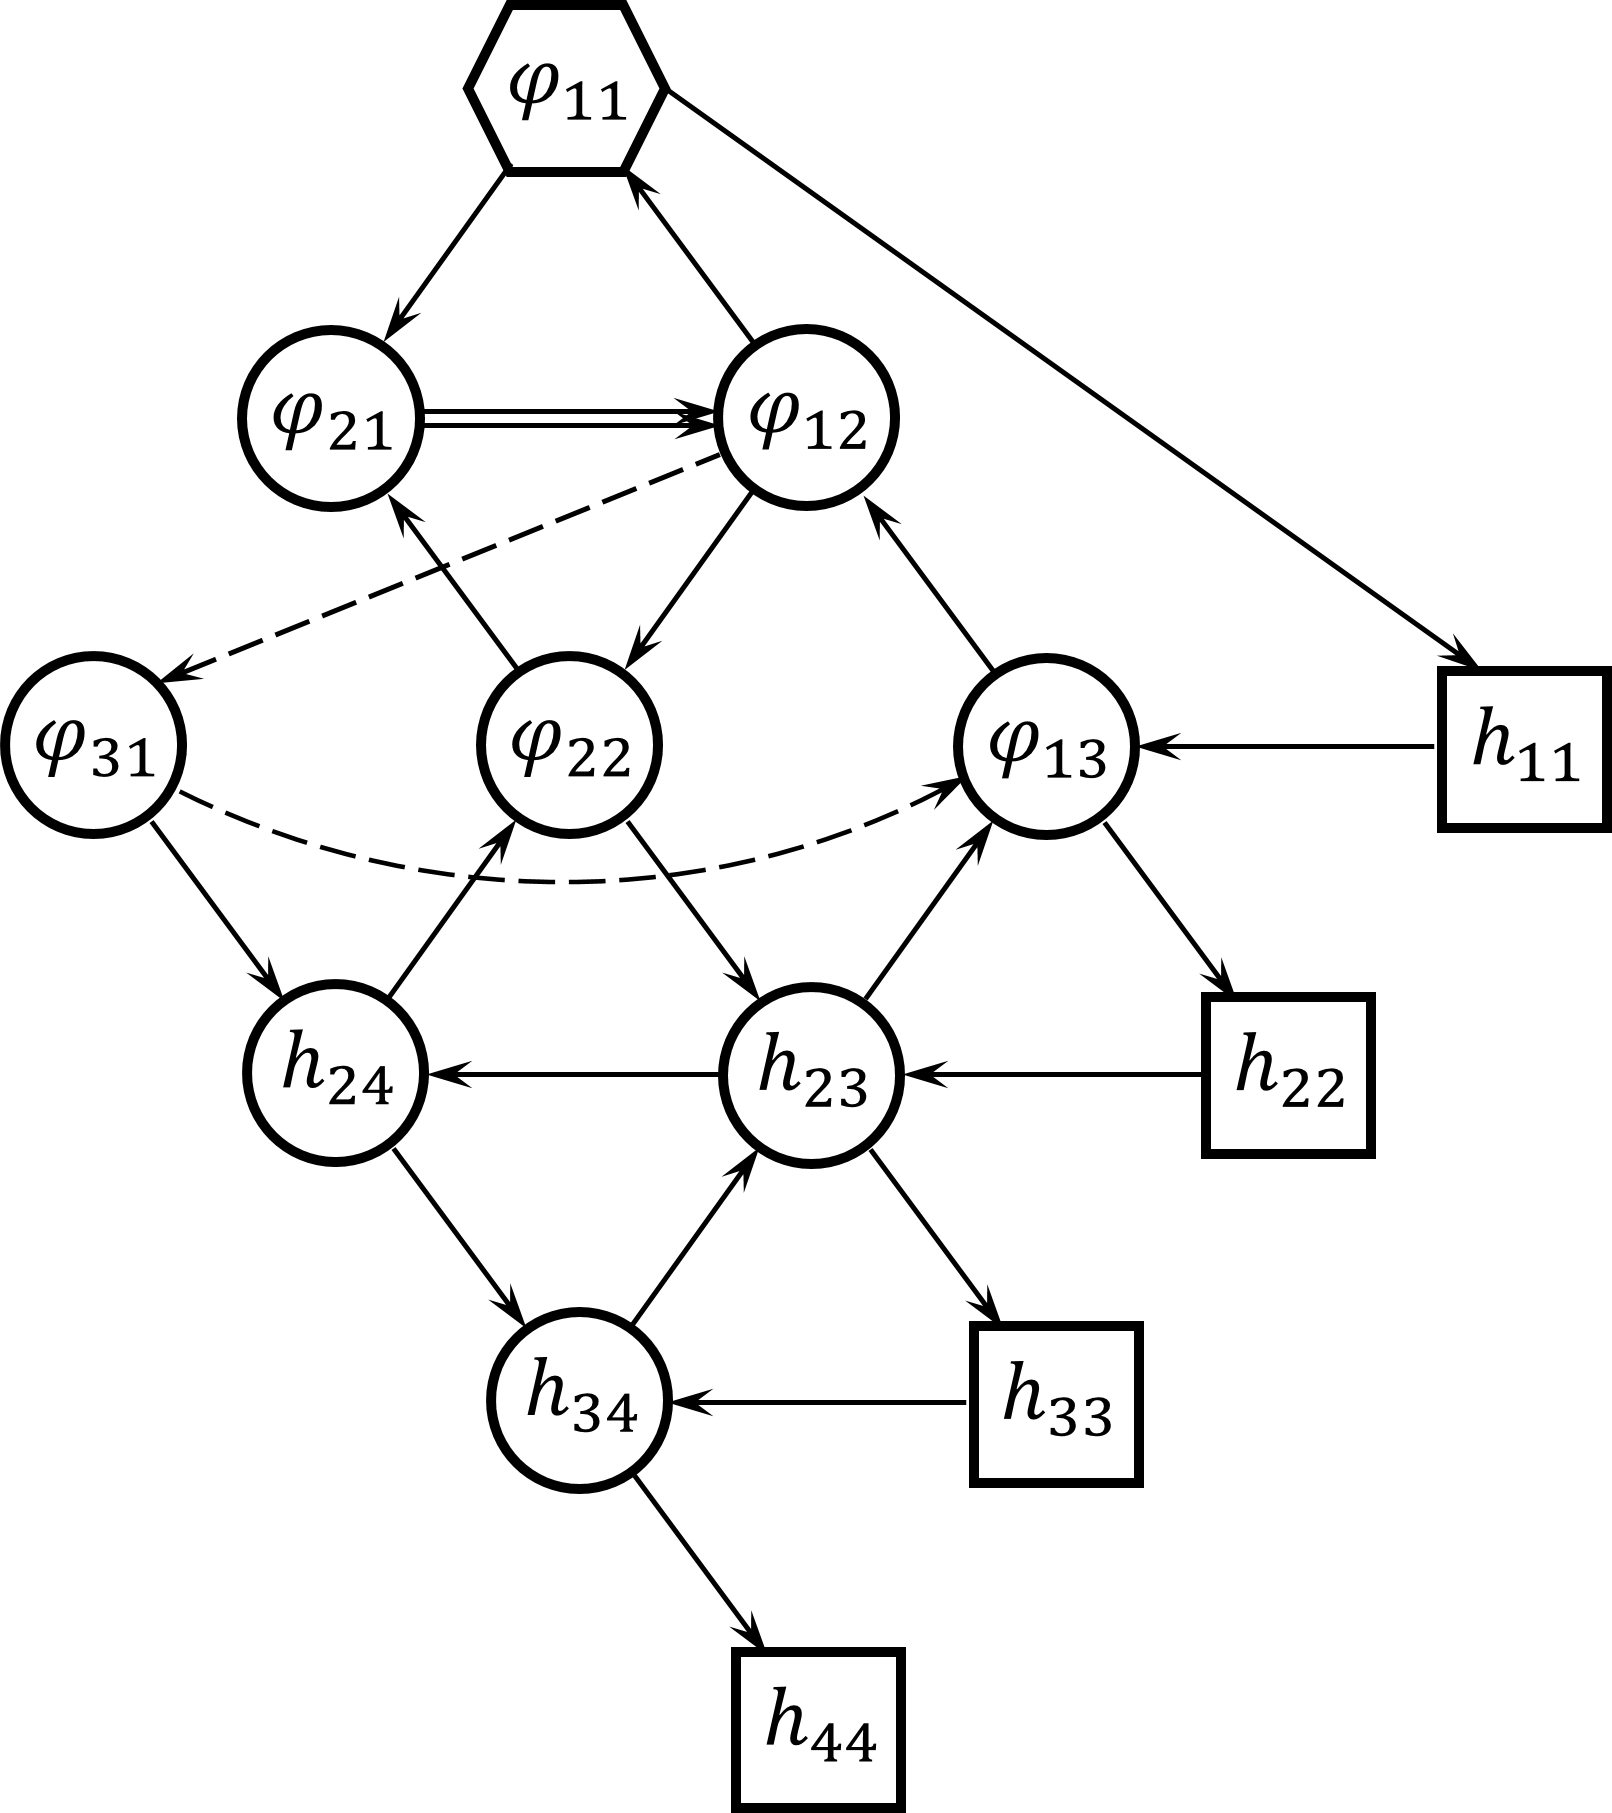
\includegraphics[scale=0.65]{h_convention/h_n=4_std.png}
\end{center}
\caption{The initial quiver for $\gc^{\dagger}_h(\bg_{\std},\GL_4)$.}
\label{f:h_n=4_std}
\end{figure}

\paragraph{The initial variables.} The $\varphi$-variables are given by
\begin{align}
    &\varphi_{11}(U) = -\det \begin{bmatrix}
        u_{14} & (U^2)_{14} & (U^3)_{14}\\
        u_{24} & (U^2)_{24} & (U^3)_{24}\\
        u_{34} & (U^2)_{34} & (U^3)_{34}
    \end{bmatrix};\\ &\varphi_{12}(U) =  \det \begin{bmatrix}
        u_{13} & u_{14} & (U^2)_{14}\\
        u_{23} & u_{24} & (U^2)_{24}\\
        u_{33} & u_{34} & (U^2)_{34}
    \end{bmatrix}, \ \ \varphi_{21}(U) = \det \begin{bmatrix}
        u_{14} & (U^2)_{14}\\ u_{24} & (U^2)_{24}
    \end{bmatrix};  \\
    &\varphi_{31}(U) = -u_{14}, \ \ \varphi_{22}(U) = \det U_{[1,2]}^{[3,4]}, \ \ \varphi_{13}(U) = - \det U_{[1,3]}^{[2,4]}.
\end{align}

The $h$-variables are given by
\begin{align}
    &h_{24}(U) = u_{24}, \ \ h_{23}(U) = \det U_{[2,3]}^{[3,4]}, \ \ h_{22}(U) = \det U_{[2,4]}^{[2,4]};\\
    &h_{34}(U) = -u_{34}, \ \ h_{33}(U) = \det U_{[3,4]}^{[3,4]}, \ \ h_{44}(U) = u_{44}.
\end{align}

The $c$-variables are given by
\begin{align}
    &c_1(U) = -\tr U, \ \ c_2(U) = \frac{1}{2!}\left(\tr(U)^2 - \tr(U^2)\right),\\ &c_3(U) = -\frac{1}{3!}\left( \tr(U)^3 - 3\tr(U)\tr(U^2)+2\tr(U^3)\right).
\end{align}

\paragraph{List of $1$-step mutations.} Here's what one obtains after a $1$-step mutation of the initial cluster in each direction:
%-U(1,4)*det(U([2,3],[1,4]))-U(3,4)*det(U([2,3],[3,4]))-U(2,4)*det(U(2:3,[2,4])) )
\begin{align}
&\varphi_{12}^\prime(U) = \det U_{[1,2]}^{[3,4]} \det \begin{bmatrix}
    u_{14} & (U^2)_{14}\\ u_{34} & (U^2)_{34} 
\end{bmatrix} + \begin{bmatrix}
    u_{14} & (U^2)_{14}\\ u_{24} & (U^2)_{24} 
\end{bmatrix} \det U_{[1,2]}^{\{2,4\}};\\
&\varphi_{21}^\prime(U) = -\det \begin{bmatrix}
    u_{14} & (U^2)_{13} & (U^2)_{14}\\
    u_{24} & (U^2)_{23} & (U^2)_{24}\\
    u_{34} & (U^2)_{33} & (U^2)_{34}
\end{bmatrix};\\
    &\varphi_{31}^\prime(U) = -\det U_{[1,3]}^{\{1\}\cup[3,4]}, \ \ 
\varphi_{31}^\prime(U) = -u_{24}\det U_{[2,4]}^{[2,4]} - u_{14} \det U_{[2,4]}^{\{1\}\cup[3,4]};\\&\varphi_{22}^\prime(U) = -u_{14}\det U_{[2,3]}^{\{1,4\}} - u_{24} \det U_{[2,3]}^{\{2,4\}} - u_{34} \det U_{[2,3]}^{[3,4]}.
\end{align}
\begin{align}
    &h_{24}^\prime(U) = -\det U_{\{1,3\}}^{[3,4]},\ \ \ h_{34}^\prime(U) = -\det U_{\{2,4\}}^{[3,4]};\\
    &h_{23}^\prime(U) = u_{14}\det U_{[2,4]}^{[2,4]} - u_{24} \det U_{\{1\}\cup[3,4]}^{[2,4]}.
\end{align}